\documentclass[12pt,aspectratio=169]{beamer}

% ====================================================
% ====================================================
% USEPACKAGES AND IMPORTS
% ====================================================
% ====================================================

\usepackage[T1]{fontenc}
\usepackage[utf8]{inputenc}
\usepackage[english]{babel}

% tables
\usepackage{tabularx}
\usepackage{colortbl}
\usepackage{multirow}
\usepackage{makecell}

% tikz and colors
\usepackage{tikz}
\usepackage{xcolor}
\usepackage{pgfplots}
\usepackage{pgfplotstable}
\usepackage{tikzsymbols}

\usetikzlibrary{calc}
\usetikzlibrary{trees}
\usetikzlibrary{patterns}
\usetikzlibrary{shadings}
\usetikzlibrary{positioning}
\usetikzlibrary{intersections}
\usepgfplotslibrary{patchplots}
\usepgfplotslibrary{fillbetween}
\usetikzlibrary{decorations.pathreplacing}

\usetikzlibrary{arrows}
\usetikzlibrary{arrows.meta}

\usetikzlibrary{shapes}
\usetikzlibrary{shapes.arrows}
\usetikzlibrary{shapes.callouts}
\usetikzlibrary{shapes.symbols}
\usetikzlibrary{shapes.geometric}

% boxes
\usepackage[many]{tcolorbox}

% math packages and fonts
\usepackage{bm}
\usepackage{ccfonts}
\usepackage{eulervm}
\usepackage{amsmath}
\usepackage{amsfonts}
\usepackage{amssymb}
\usepackage{amsthm}
\usepackage{mathtools}
\usepackage{nicefrac}
\usepackage{slashed}
\usepackage{bbold}
\usepackage{array}
\usepackage{cancel}

% algorithms and listings
\usepackage[ruled,vlined,linesnumbered]{algorithm2e}
\usepackage{listings}
\usepackage{setspace}

\tcbuselibrary{listings}
\tcbuselibrary{breakable}
\tcbuselibrary{skins}

% misc
\usepackage{soul}
\usepackage{pifont}
\usepackage{skull}
\usepackage{multicol}
\usepackage{animate}
\usepackage{hyperref}
\usepackage{wasysym}
\usepackage[absolute,overlay]{textpos}
\usepackage[hang,flushmargin]{footmisc}

% ====================================================
% ====================================================
% LAYOUT AND THEME
% ====================================================
% ====================================================

\usetheme{Copenhagen}

% color definitions
\definecolor{myblue1}{RGB}{35,119,189}
\definecolor{myblue2}{RGB}{95,179,238}
\definecolor{myblue3}{RGB}{129,168,207}
\definecolor{myblue4}{RGB}{26,89,142}

\definecolor{myred1}{RGB}{247,12,12}

% set theme colors
\setbeamercolor*{structure}{fg=myblue1,bg=blue}
\setbeamercolor*{palette primary}{use=structure,fg=white,bg=structure.fg}
\setbeamercolor*{palette secondary}{use=structure,fg=white,bg=structure.fg!75!black}
\setbeamercolor*{palette tertiary}{use=structure,fg=white,bg=structure.fg!50!black}
\setbeamercolor*{palette quaternary}{fg=black,bg=white}

\setbeamertemplate{itemize item}[circle]
\setbeamertemplate{itemize subitem}[circle]
\setbeamertemplate{itemize subsubitem}[circle]

\setbeamertemplate{enumerate item}[circle]
\setbeamertemplate{enumerate subitem}[circle]
\setbeamertemplate{enumerate subsubitem}[circle]

\setbeamercolor{itemize item}{fg=myblue1}
\setbeamercolor{itemize subitem}{fg=myblue1}
\setbeamercolor{itemize subsubitem}{fg=myblue1}

\setbeamertemplate{section in toc}[circle]
\setbeamertemplate{subsection in toc}[circle]
\setbeamerfont{subsection in toc}{size=\scriptsize}

\setbeamercolor{frametitle continuation}{fg=black}

% title graphic -- sap logo and dhbw logo
\titlegraphic{
\includegraphics[scale=0.1]{../03_img/logo_sap}\hspace*{4.75cm}~%
   	
\includegraphics[scale=0.05]{../03_img/logo_dhbw}
}

\makeatletter
% frame title
\defbeamertemplate*{frametitle}{mydefault}[1][left]
{
  	\ifbeamercolorempty[bg]{frametitle}{}{\nointerlineskip}%
  	\nointerlineskip%
 	\@tempdima=\textwidth%
  	\advance\@tempdima by\beamer@leftmargin%
  	\advance\@tempdima by\beamer@rightmargin%
  	\begin{tcolorbox}[
  		enhanced,
  		outer arc=0pt,
  		arc=0pt,
  		boxrule=0pt,
  		top=0pt,
  		bottom=0pt,
  		enlarge left by=-\beamer@leftmargin,
  		enlarge right by=-\beamer@rightmargin,
  		width=\paperwidth,
  		nobeforeafter,
  		interior style={
    			left color=myblue2,
    			right color=white
    		},
  		shadow={0mm}{-0.4mm}{0mm}{black!60,opacity=0.6},    
  		shadow={0mm}{-0.8mm}{0mm}{black!40,opacity=0.4},    
  	]
    	\usebeamerfont{frametitle}%
    	\vbox{}\vskip-1ex%
    	\if@tempswa\else\csname beamer@fte#1\endcsname\fi%
    	\insertframetitle\par%
    	{%
      		\ifx\insertframesubtitle\@empty%
      		\else%
      		{\usebeamerfont{framesubtitle}\usebeamercolor[fg]{black}\insertframesubtitle\strut\par}%
      		\fi
    	}%
    	\vskip-1ex%
    	\if@tempswa\else\vskip-.3cm\fi
  	\end{tcolorbox}%
}

% footline of a frame
\defbeamertemplate*{footline}{mysplit theme}
{%
  	\leavevmode%
  	\hbox{
		\begin{beamercolorbox}[
			wd=.5\paperwidth,ht=2.5ex,dp=1.125ex,leftskip=.3cm plus1fill,rightskip=.3cm
		]{author in head/foot}%
    			\usebeamerfont{author in head/foot}\insertshortauthor\ (\insertinstitute), \insertdate
  		\end{beamercolorbox}%
  		\begin{beamercolorbox}[
			wd=.5\paperwidth,ht=2.5ex,dp=1.125ex,leftskip=.3cm,rightskip=.3cm plus1fil
		]{title in head/foot}%
    			\usebeamerfont{title in head/foot}\insertshorttitle\hfill
    			\insertprefix-\insertframenumber/\inserttotalframenumber\hspace*{0.5em}
  		\end{beamercolorbox}}%
  	\vskip0pt%
}
\makeatother

% ====================================================
% ====================================================
% COMMANDS AND GENERAL DEFINITIONS
% ====================================================
% ====================================================

% page number prefix
\newcommand\insertprefix{}  % empty by default
\newcommand\prefix[1]{\renewcommand\insertprefix{#1}}

% math definitions
% ====================================================
\DeclareMathOperator*{\argmax}{arg\,max}
\DeclareMathOperator*{\argmin}{arg\,min}
\newcommand*\diff{\mathop{}\!\mathrm{d}}

\newcommand*{\vertbar}{\rule[-1ex]{0.5pt}{2.5ex}}
\newcommand*{\horzbar}{\rule[.5ex]{2.5ex}{0.5pt}}

% commands
% ====================================================

% highlight commands
% --------------------------------------------------------------------------------------------------------
% highlight command
\newcommand{\highlight}[1]{\textcolor{myblue1}{\textbf{#1}}}
\newcommand{\highlighttt}[1]{\textcolor{myblue1}{\texttt{#1}}}
\newcommand{\Highlight}[1]{\textcolor{myred1}{\textbf{#1}}}

% blue color boxes (with frame/without frame/without fill)
\newtcolorbox{boxBlue}{colback=myblue1!10!white,colframe=myblue4}
\newtcolorbox{boxBlueNoFrame}{colback=myblue1!10!white,colframe=myblue1!10!white}
\newtcolorbox{boxBlueNoFill}{colback=white,colframe=myblue4}

% font commands
% --------------------------------------------------------------------------------------------------------
\newcommand{\linkstyle}[1]{\underline{\smash{\texttt{#1}}}} 		% style of hyperlinks

% tikz commands
% --------------------------------------------------------------------------------------------------------

% yellow sticky note
\newcommand{\bubble}[3]{
\begin{textblock}{100}(#1, #2)
      	\begin{tikzpicture}
		\node[rectangle,draw=yellow,very thick,fill=yellow!60,align=center] at (0,0) {#3};
	\end{tikzpicture}
\end{textblock}
}

\newcommand{\floattext}[3]{
\begin{textblock}{100}(#1, #2)
      	#3
\end{textblock}
}

\newcommand{\doublecircle}[2]{
	\draw[fill=white,draw=myblue1] (#1,#2) circle (2mm);
	\draw[fill=myblue1,draw=myblue1] (#1,#2) circle (1.5mm);
}

% slide modifiers
% --------------------------------------------------------------------------------------------------------
% mark slide as optional
\newcommand{\optional}{
	\begin{textblock}{100}(0.15,0.30)
      		
\includegraphics[scale=0.2]{../03_img/scream}
    	\end{textblock}
}

% mark slide as important
\newcommand{\important}{
	\begin{textblock}{100}(0.10,0.15)
      		
\includegraphics[scale=0.1]{../03_img/important}
    	\end{textblock}
}

% citation
% --------------------------------------------------------------------------------------------------------
% first argument in {book, online, article}
\newcommand{\literature}[5]{
	\setbeamertemplate{bibliography item}[#1]
	\bibitem{#2}
	\highlight{#3} \\
	\textcolor{darkgray}{\textit{#4}} \\
	\textcolor{black}{#5}
}
% cite content
\newcommand{\citeAuthor}[3]{\vfill\scriptsize\textcolor{lightgray}{#1 \cite{#2} #3}}

% slide architecture
% --------------------------------------------------------------------------------------------------------
% divide frame into two parts
\newcommand{\divideTwo}[4]{
	\begin{minipage}{#1\textwidth}
		#2
	\end{minipage}
	\hfill
	\begin{minipage}{#3\textwidth}
		#4
	\end{minipage}
}

% divide frame into two parts (start on top)
\newcommand{\divideTwoTop}[4]{
	\begin{minipage}[t]{#1\textwidth}
		#2
	\end{minipage}
	\hfill
	\begin{minipage}[t]{#3\textwidth}
		#4
	\end{minipage}
}

% special pages
% --------------------------------------------------------------------------------------------------------
% title page
\newcommand{\maketitlepage}{
	{
		\beamertemplatenavigationsymbolsempty
		\usebackgroundtemplate{%
			\tikz[overlay,remember picture] \node[opacity=0.2, at=(current page.center)] {
  				
\includegraphics[height=\paperheight,width=\paperwidth]{../03_img/processor.jpg}
			};
		}
		\begin{frame}[plain]
			\vspace*{0.75cm}
			\maketitle
			\vfill
			\begin{center}
				\footnotesize Find all slides on \href{https://github.com/DaWe1992/Applied_ML_Fundamentals}{\linkstyle{GitHub}}
			\end{center}
		\end{frame}
	}
}

% divider page
\newcommand{\makedivider}[1]{
	{
		\beamertemplatenavigationsymbolsempty
		\usebackgroundtemplate{%
			\tikz[overlay,remember picture] \node[opacity=0.2, at=(current page.center)] {
  				
\includegraphics[height=\paperheight,width=\paperwidth]{../03_img/processor.jpg}
			};
		}
		\begin{frame}[plain]
			\vfill
			\begin{boxBlue}
				\centering
				\textbf{Section:} \\
				\large \highlight{#1}
			\end{boxBlue}
			\vfill
			\centering
			
\includegraphics[scale=0.05]{../03_img/logo_dhbw.png}
			\vfill
		\end{frame}
	}
}

% overview page
\newcommand{\makeoverview}[1]{
	\begin{frame}{Lecture Overview}{}
		\begin{tabbing}
			\hspace*{3.5cm}\= \kill
			\ifnum #1=1 \highlight{\textbf{Unit I:}} \else \textbf{Unit I:} \fi
			\> \ifnum #1=1 \highlight{Machine Learning Introduction} \else Machine Learning Introduction \fi \\
		\end{tabbing}
	\end{frame}
}

% thank you page
\newcommand{\makethanks}{
	{\beamertemplatenavigationsymbolsempty
	\begin{frame}[plain]
		\vfill
		\begin{boxBlue}
			\centering
			\Large \highlight{Thank you very much for the attention!}
		\end{boxBlue}
		
		\vfill\footnotesize
		\begin{tabbing}
			\hspace*{1.5cm}\= \kill
			\highlight{Topic:} 	\> \inserttitle \\
			\highlight{Date:} 	\> \insertdate
		\end{tabbing}
		
		\vfill
		\highlight{Contact:} \\
		\insertauthor\ (D062271) \\
		\insertinstitute \\
		\href{mailto:daniel.wehner@sap.com}{\linkstyle{daniel.wehner@sap.com}}
		
		\vfill\normalsize
		\begin{center}
			\large\highlight{Do you have any questions?}
		\end{center}
		\vfill
	\end{frame}}
}

% global pfgplots settings
% --------------------------------------------------------------------------------------------------------
\pgfplotsset{
	% allow filtering of data for pgfplots
	discard if/.style 2 args={
        		x filter/.code={
            		\edef\tempa{\thisrow{#1}}
            		\edef\tempb{#2}
            		\ifx\tempa\tempb
                		\def\pgfmathresult{inf}
            		\fi
        		}
    	},
    	discard if not/.style 2 args={
        		x filter/.code={
            		\edef\tempa{\thisrow{#1}}
            		\edef\tempb{#2}
            		\ifx\tempa\tempb
            		\else
                		\def\pgfmathresult{inf}
            		\fi
        		}
    	}
}


% ====================================================
% ====================================================
% PRESENTATION DATA
% ====================================================
% ====================================================

\title[Probabilistic Graphical Models]{*** Applied Machine Learning Fundamentals *** Probabilistic Graphical Models}
\institute{SAP\,SE}
\author{M.\,Sc. Daniel Wehner}
\date{Winter term 2019/2020}
\prefix{PGM}

% ====================================================
% ====================================================
% BEGIN OF DOCUMENT
% ====================================================
% ====================================================

\begin{document}

% Title frame
%______________________________________________________________________
\maketitlepage


% Lecture Overview
%______________________________________________________________________
\begin{frame}{Lecture Overview}{}
	\begin{center}
		\Huge\highlight{Out of scope for this lecture!}
	\end{center}
\end{frame}


% Agenda
%______________________________________________________________________
\begin{frame}{Agenda for this Unit}
	\begin{multicols}{2}
		\tableofcontents
	\end{multicols}
\end{frame}


% Section: Introduction
%______________________________________________________________________
\section{Basic Statistics}
\makedivider{Basic Statistics}

% Subsection: Random Variables and Probability Distributions
% --------------------------------------------------------------------------------------------------------
\subsection{Random Variables and Probability Distributions}

% Random Variables and Probability Distributions
\begin{frame}{Random Variables and Probability Distributions}{}
	\begin{itemize}
		\item What is a random variable $X$? \\
			\highlight{A random number whose value is subject to variations due to chance}
		\item What is a distribution $p(X = x_i)$? \\
			\highlight{Describes the probability (density) that the random variable $X$ will be equal to a certain value $x_i$}
		\item What is a joint, a conditional and a marginal distribution?  \\
			\highlight{$\underbracket{p(X, Y)}_{\text{joint}} = \underbracket{p(Y \vert X)}_{\text{cond.}} \cdot
			\underbracket{p(X)}_{\text{marg.}}$}
	\end{itemize}
\end{frame}


% Subsection: Important Probability Rules
% --------------------------------------------------------------------------------------------------------
\subsection{Important Probability Rules}

% Important Probability Rules
\begin{frame}{Important Probability Rules}{}
	\begin{itemize}
		\item \highlight{Bayes' rule}
		\begin{equation}
			p(X \vert Y) = \frac{p(Y \vert X) \cdot p(X)}{p(Y)}
		\end{equation}
		\item \highlight{Chain rule of probabilities}
		\begin{equation}
			p(W, X, Y, Z) = p(W \vert X, Y, Z) \cdot p(X \vert Y, Z) \cdot p(Y \vert Z) \cdot p(Z)
		\end{equation}
		\item \highlight{Definition of conditional probability}
		\begin{equation}
			p(X \vert Y) = \frac{p(X, Y)}{p(Y)}
		\end{equation}
	\end{itemize}
\end{frame}


% Section: Bayesian Networks
%______________________________________________________________________
\section{Bayesian Networks (BNs)}
\makedivider{Bayesian Networks (BNs)}

% Subsection: Representation of large Probability Distributions
% --------------------------------------------------------------------------------------------------------
\subsection{Representation of large Probability Distributions}

% Representing Distributions by Enumeration
\begin{frame}{Representing Distributions by Enumeration}{}
	\begin{itemize}
		\item Consider a probability distribution $p(X)$
		\begin{itemize}
			\item Assign a probability to each $x_i \in Dom(X)$
			\item Q: How many parameters do we have? (assuming $\vert Dom(X) \vert = k$)
			\item A: \highlight{$k - 1$} (Remember: $\sum_{x_i \in Dom(X)} p(x_i) = 1$)
		\end{itemize}
		\item Now consider $p(X_1, X_2, \dots, X_n)$
		\begin{itemize}
			\item Q: How many parameters do we have now?
			\item A: \highlight{$k^n - 1$} \Highlight{(Exponentially many!)}
		\end{itemize}
	\end{itemize}

	\begin{boxBlueNoFrame}
		\highlight{Bayesian networks often need much fewer parameters. Why?}
	\end{boxBlueNoFrame}
\end{frame}


% Simple Bayesian Network (2 Nodes)
\begin{frame}{Simple Bayesian Network (2 Nodes)}{}
	\divideTwo{0.44}{
		\begin{itemize}
			\item Let's first consider a simple BN
			\item Grade $G$ is influenced by intelligence $I$
		\end{itemize}

		\begin{figure}
	\centering
	\begin{tikzpicture}[
		scale=0.8
	]

		\node[circle,draw=black] (I) at (0,1) {$I$}; \node[align=left,text width=1cm] at (1.5,1) {\tiny $\in \{hi, lo\}$};
		\node[circle,draw=black] (G) at (0,-1) {$G$}; \node[align=left,text width=1cm] at (1.5,-1) {\tiny $\in \{a, b\}$};
		\draw[->] (I) -- (G);
		
		\node at (-1.5,1) {\tiny rand. variable};
		\node at (1,0) {\tiny `influences'};
	\end{tikzpicture}
\end{figure}
	}{0.54}{
		\begin{table}[h]
	\scalebox{0.8}{
		\renewcommand{\arraystretch}{1.0}
		\begin{tabular}{| c || c | c |}
			\hline
			&
			$I = hi$ &
			$I = lo$ \\
			\hline\hline
			$p(I)$	&	0.85	&	0.15 \\
			\hline
		\end{tabular}
	}
\end{table}














		\vspace*{-5mm}
		\begin{table}[h]
	\scalebox{0.8}{
		\renewcommand{\arraystretch}{1.0}
		\begin{tabular}{| c || c | c | c |}
			\hline
			& 
			$G$	&
			$I = hi$ &
			$I = lo$ \\
			\hline\hline
			\multirow{2}{*}{$p(G \vert I)$}	&	a 	&	0.90	&	0.50 \\
									&	b 	&	0.10	&	0.50 \\
			\hline
		\end{tabular}
	}
\end{table}















		\footnotesize
		\begin{align*}
			p(G = b, I = h) 	&\overset{CR}{=} p(G = b \vert I = hi) \cdot p(I = hi) \\
						&= 0.85 \cdot 0.1 = \bm{0.085}
		\end{align*}
	}
\end{frame}


% What if Variables are independent?
\begin{frame}{What if Variables are independent?}{}
	\begin{itemize}
		\item Random variables: Intelligence $I$, Grade $G$, SAT score $S$
		\begin{figure}
	\centering
	\begin{tikzpicture}[
		scale=0.8
	]

		\node[circle,draw=black] (I) at (0,1) {$I$}; \node at (1.25,1) {$p(I)$};
		\node[circle,draw=black] (G) at (-1.5,-1) {$G$}; \node at (-3,-1) {$p(G \vert I)$};
		\node[circle,draw=black] (S) at (1.5,-1) {$S$}; \node at (3,-1) {$p(S \vert I)$};
		\draw[->] (I) -- (G);
		\draw[->] (I) -- (S);

	\end{tikzpicture}
\end{figure}
		\item $G$ and $S$ are influenced by $I$
		\item \textbf{But:} $G$ is independent of $S$ given $I$: $G \indep S \vert I$
		\item \highlight{Independencies can lead to a smaller number of parameters}
	\end{itemize}
\end{frame}


% Can we get linear Complexity?
\begin{frame}{Can we get linear Complexity?}{}
	\begin{itemize}
		\item \textbf{Yes we can!}
		\item But we must assume $(\bm{X} \indep \bm{Y})\ \forall\ \bm{X}, \bm{Y}$ subsets of $\{X_1, X_2, \dots, X_m\}$
		\item The joint probability distribution can be written as:
		\begin{equation}
			p(X_1, X_2, \dots, X_n) = \prod_{j=1}^m p(X_j)
		\end{equation}
		\item Q: How many parameters do we have? A: $m \cdot (k - 1) = \mathcal{O}(m)$
		\begin{figure}
	\centering
	\begin{tikzpicture}[
		scale=0.8
	]

		\node[circle,draw=black] at (-4,0) {$X_1$};
		\node[circle,draw=black] at (-2,0) {$X_2$};
		\node[circle,draw=black] at (0,0) {$X_3$};
		\node at (2,0) {$\dots$};
		\node[circle,draw=black] at (4,0) {$X_m$};

	\end{tikzpicture}
\end{figure}
	\end{itemize}
\end{frame}


% Na\"{i}ve Bayes
\begin{frame}{Na\"{i}ve Bayes}{}
	\begin{itemize}
		\item This leads to the Na\"{i}ve Bayes model
		\item Class variable $C$, evidence variables $\{X_1, X_2, \dots, X_m\}$
		\item Assume: $(\bm{X} \indep \bm{Y} \vert C) \ \forall\ \bm{X}, \bm{Y}$ subsets of $\{X_1, X_2, \dots, X_m\}$
		\begin{figure}
	\centering
	\begin{tikzpicture}[
		scale=0.6,
		every node/.style={scale=0.6}
	]

		\node[circle,draw=black] (C) at (0,2) {$C$};
		\node[circle,draw=black] (X1) at (-4,0) {$X_1$};
		\node[circle,draw=black] (X2) at (-2,0) {$X_2$};
		\node[circle,draw=black] (X3) at (0,0) {$X_3$};
		\node (Xi) at (2,0) {$\dots$};
		\node[circle,draw=black] (Xm) at (4,0) {$X_m$};
		\draw[->] (C) -- (X1);
		\draw[->] (C) -- (X2);
		\draw[->] (C) -- (X3);
		\draw[->,dashed] (C) -- (Xi);
		\draw[->] (C) -- (Xm);
		
	\end{tikzpicture}
\end{figure}
		\begin{equation}
			p(X_1, X_2, \dots, X_m, C) = p(C) \cdot \prod_{j=1}^m p(X_j \vert C)
		\end{equation}
	\end{itemize}
	\textcolor{gray}{$\Rightarrow$ cf. slides `Decision Theory'}
\end{frame}


% Local Markov Assumption
\begin{frame}{Local Markov Assumption}{}
	\begin{itemize}
		\item How to read off the independencies from a BN?
		\item \highlight{Local Markov assumption}: A variable is independent of its non-descendants given its parents
			and only its parents:
		\begin{equation}
			(X_j \indep \underbracket{NonDescendants(X_j)}_{ND(X_j)} \vert \underbracket{Parents(X_j)}_{Pa(X_j)})\
			\forall\ j = 1, 2, \dots, m
		\end{equation}
	\end{itemize}
	\textcolor{gray}{$\Rightarrow$ cf. examples on the next slide}
\end{frame}


% Example: Local Markov Assumption
\begin{frame}{Example: Local Markov Assumption}{}
	\divideTwo{0.49}{
		\begin{figure}
	\centering
	\begin{tikzpicture}[
		scale=0.8
	]

		\node[circle,draw=black] (A) at (-1.5,2) {$A$}; \node at (-1.5,3) {\footnotesize \textit{Allergy}};
		\node[circle,draw=black] (F) at (1.5,2) {$F$}; \node at (1.5,3) {\footnotesize \textit{Flu}};
		\node[circle,draw=black] (S) at (0,0) {$S$}; \node at (1.25,0) {\footnotesize \textit{Sinus}};
		\node[circle,draw=black] (N) at (-1.5,-2) {$N$}; \node at (-1.5,-3) {\footnotesize \textit{Runny Nose}};
		\node[circle,draw=black] (H) at (1.5,-2) {$H$}; \node at (1.5,-3) {\footnotesize \textit{Headache}};

		\draw[->] (A) -- (S);
		\draw[->] (F) -- (S);
		\draw[->] (S) -- (N);
		\draw[->] (S) -- (H);

	\end{tikzpicture}
\end{figure}
	}{0.49}{
		\scriptsize
		\begin{boxBlueNoFrame}
			\vspace*{-6mm}
			\begin{align*}
				Pa(F) 		&= \emptyset \\
				ND(F) 		&= \{A\} \\
				Independencies	&\Rightarrow (F \indep A)
			\end{align*}
			\vspace*{-8mm}
		\end{boxBlueNoFrame}

		\begin{boxBlueNoFrame}
			\vspace*{-6mm}
			\begin{align*}
				Pa(N) 		&= \{S\} \\
				ND(N) 		&= \{F, A, H\} \\
				Independencies	&\Rightarrow (N \indep \{F, A, H\} \vert S)
			\end{align*}
			\vspace*{-8mm}
		\end{boxBlueNoFrame}

		\begin{boxBlueNoFrame}
			\vspace*{-6mm}
			\begin{align*}
				Pa(S) 		&= \{F, A\} \\
				ND(S) 		&= \emptyset \\
				Independencies	&\Rightarrow\ \text{none} 
			\end{align*}
			\vspace*{-8mm}
		\end{boxBlueNoFrame}
	}
\end{frame}


% Explaining away / Berkson's Paradox
\begin{frame}{Explaining away / Berkson's Paradox}{}
	\divideTwo{0.49}{
		\begin{figure}
	\centering
	\begin{tikzpicture}[
		scale=0.8
	]

		\node[circle,draw=black] (A) at (-1.5,2) {$A$}; \node at (-1.5,3) {\footnotesize \textit{Allergy}};
		\node[circle,draw=black] (F) at (1.5,2) {$F$}; \node at (1.5,3) {\footnotesize \textit{Flu}};
		\node[circle,draw=black,fill=black,text=white] (S) at (0,0) {$S$}; \node at (1.25,0) {\footnotesize \textit{Sinus}};
			\node at (-1.5,0) {\scriptsize \textit{`observed'}};
		\node[circle,draw=black] (N) at (-1.5,-2) {$N$}; \node at (-1.5,-3) {\footnotesize \textit{Runny Nose}};
		\node[circle,draw=black] (H) at (1.5,-2) {$H$}; \node at (1.5,-3) {\footnotesize \textit{Headache}};

		\draw[->] (A) -- (S);
		\draw[->] (F) -- (S);
		\draw[->] (S) -- (N);
		\draw[->] (S) -- (H);

	\end{tikzpicture}
\end{figure}
	}{0.49}{
		\begin{itemize}
			\item Two causes ($A$, $F$) `compete' to explain the observed data ($S$)
			\item \textbf{Having a flu makes it less likely to have an allergy}
			\item It follows: $\neg(F \indep A \vert S)$, although $F \indep A$ (!!!)
			\item This is \textbf{not} implied by the local Markov assumption \\
				(S is descendant not parent!)
		\end{itemize}
	}
\end{frame}


% Joint Distribution
\begin{frame}{Joint Distribution}{}
	\begin{itemize}
		\item According to the \textbf{chain rule} the joint probability distribution $P(A, F, S, H, N)$ is given by:
		\begin{equation*}
			p(A, F, S, H, N) = p(F) \cdot p(A \vert F) \cdot p(S \vert F, A) \cdot p(H \vert S, F, A) \cdot p(N \vert S, F, A, H)
		\end{equation*}
		\item Apply independency assumptions (\textbf{local Markov assumption}):
		\begin{equation*}
			p(A, F, S, H, N) = p(F) \cdot p(A) \cdot p(S \vert F, A) \cdot p(H \vert S) \cdot p(N \vert S)
		\end{equation*}
	\end{itemize}

	\vspace*{-3mm}
	\begin{boxBlueNoFrame}
		\highlight{Much less parameters due to the local Markov assumption!}
	\end{boxBlueNoFrame}
\end{frame}


% Definition of a Bayesian Network
\begin{frame}{Definition of a Bayesian Network}{}
	\begin{itemize}
		\item A BN is a \textbf{directed acyclic graph (DAG)}
		\begin{itemize}
			\item Nodes represent random variables $\{X_1, X_2, \dots, X_m\}$
			\item Edges represent the dependencies between the random variables
		\end{itemize}
		\item Due to the \textbf{local Markov assumption} the joint probability distribution factorizes according to:
	\end{itemize}

	\begin{boxBlue}
		\begin{equation}
			\large
			p(X_1, X_2, \dots, X_m) = \prod_{j=1}^m p(X_j \vert Pa(X_j))
		\end{equation}
	\end{boxBlue}
\end{frame}


% Independencies in real Problems
\begin{frame}{Independencies in real Problems}{}
	\divideTwo{0.49}{
		\begin{boxBlueNoFill}
			\vfill
			\begin{center}
				\large \textbf{Real world} \\
				\vspace*{3mm}
				
\includegraphics[scale=0.03]{15_pgm/02_img/earth} \\
				\vspace*{2mm}
				{\footnotesize The true distribution $P$ contains independency assertions $I(P)$}
			\end{center}
			\vfill
		\end{boxBlueNoFill}
	}{0.49}{
		\begin{boxBlueNoFill}
			\vfill
			\begin{center}
				\large \textbf{Model} \\
				\vspace*{3mm}
				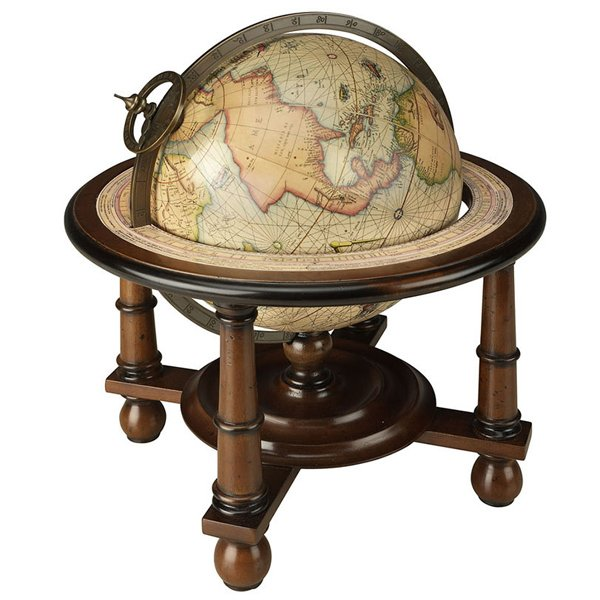
\includegraphics[scale=0.1]{15_pgm/02_img/globe} \\
				\vspace*{2mm}
				{\footnotesize The graph $\mathcal{G}$ encodes local independency assumptions $I_{LM}(\mathcal{G})$}
			\end{center}
			\vfill
		\end{boxBlueNoFill}
	}
\end{frame}


% Representation Theorem
\begin{frame}{Representation Theorem}{}
	\begin{itemize}
		\item \textbf{Key representational assumption:} $I_{LM}(\mathcal{G}) \subseteq I(P)$
		\item We say: Graph $\mathcal{G}$ is an \highlight{I-Map (independency map)} for distribution $P$
		\item \highlight{Representation theorem}:
	\end{itemize}

	\begin{center}
		\footnotesize
		\textit{Conditional independencies encoded in BN are subset of conditional independencies in $P$ \\
			$\Leftrightarrow$ \\
			Joint probability distribution factorizes according to BN definition}
	\end{center}

	\vspace*{-4mm}
	\begin{equation}
		I_{LM}(\mathcal{G}) \subseteq I(P) \Leftrightarrow P(X_1, X_2, \dots, X_m) = \prod_{j=1}^m P(X_j \vert Pa(X_j))
	\end{equation}
\end{frame}


% Independencies encoded in a BN
\begin{frame}{Independencies encoded in a BN}{}
	\begin{itemize}
		\item To get the independencies, all you need is the \textbf{local Markov assumption}
		\item But there are more... Consider the following BN:
		\vspace*{1mm}
		\begin{figure}
	\centering
	\begin{tikzpicture}[
		scale=0.8
	]

		\node[circle,draw=black] (A) at (-3,0) {$A$};
		\node[circle,draw=black] (B) at (-1,0) {$B$};
		\node[circle,draw=black] (C) at (1,0) {$C$};
		\node[circle,draw=black] (D) at (3,0) {$D$};

		\draw[->] (A) -- (B);
		\draw[->] (B) -- (C);
		\draw[->] (C) -- (D);

	\end{tikzpicture}
\end{figure}
		\vspace*{1mm}
		\item By local Markov assumption: $D \indep \{A, B\} \vert C$
		\item But we also have $D \indep A \vert C$ and $D \indep B \vert C$
			{\footnotesize (not covered by local Markov assumption)}
		\item This leads us to the concept of \highlight{d-separation (dependency separation)}
	\end{itemize}
\end{frame}


% d-Separation
\begin{frame}{d-Separation}{}
	\divideTwo{0.49}{
	 	\highlight{\circled{1} Indirect causal effect}
		\begin{figure}
	\centering
	\begin{tikzpicture}[
		scale=0.8
	]

		\node[circle,draw=black] (X) at (-3,0) {$X$};
		\node[circle,draw=black] (Z) at (-1,0) {$Z$};
		\node[circle,draw=black] (Y) at (1,0) {$Y$};

		\draw[->] (X) -- (Z);
		\draw[->] (Z) -- (Y);
		
	\end{tikzpicture}
\end{figure}
	}{0.49}{
		\highlight{\circled{2} Indirect evidential effect}
		\begin{figure}
	\centering
	\begin{tikzpicture}[
		scale=0.8
	]

		\node[circle,draw=black] (X) at (-3,0) {$X$};
		\node[circle,draw=black] (Z) at (-1,0) {$Z$};
		\node[circle,draw=black] (Y) at (1,0) {$Y$};

		\draw[->] (Y) -- (Z);
		\draw[->] (Z) -- (X);
		
	\end{tikzpicture}
\end{figure}
	}

	\vfill
	\divideTwo{0.49}{
		\highlight{\circled{3} Common cause}
		\begin{figure}
	\centering
	\begin{tikzpicture}[
		scale=0.8
	]

		\node[circle,draw=black] (X) at (-2,-1) {$X$};
		\node[circle,draw=black] (Y) at (2,-1) {$Y$};
		\node[circle,draw=black] (Z) at (0,0) {$Z$};

		\draw[->] (Z) -- (X);
		\draw[->] (Z) -- (Y);
		
	\end{tikzpicture}
\end{figure}
	}{0.49}{
		\highlight{\circled{4} Common effect (v-structure)}
		\begin{figure}
	\centering
	\begin{tikzpicture}[
		scale=0.8
	]

		\node[circle,draw=black] (X) at (-2,0) {$X$};
		\node[circle,draw=black] (Y) at (2,0) {$Y$};
		\node[circle,draw=black] (Z) at (0,-1) {$Z$};

		\draw[->] (X) -- (Z);
		\draw[->] (Y) -- (Z);

	\end{tikzpicture}
\end{figure}
	}
\end{frame}


% d-Separation (Ctd.)
\begin{frame}{d-Separation (Ctd.)}{}
	\begin{itemize}
		\item For patterns \circled{1}, \circled{2} and \circled{3} it holds:
		\begin{align*}
			X &\indep Y \vert Z \\
			\neg (X &\indep Y)
		\end{align*}
		\item Pattern \circled{4} is different (inverted):
		\begin{align*}
			X &\indep Y \\
			\neg (X &\indep Y \vert Z)
		\end{align*}
	\end{itemize}

	\begin{textblock}{100}(10.50,5.00)
      		\footnotesize
		\circled{1} indirect causal effect \\
		\circled{2} indirect evidential effect \\
		\circled{3} common cause \\
		\circled{4} common effect
    	\end{textblock}

	\begin{textblock}{100}(10.50,11.00)
      		\footnotesize
		There is an \highlight{active trail} \\
		between $X$ and $Y$, if $X$ and $Y$ \\
		are \textbf{dependent}.
    	\end{textblock}
\end{frame}


% d-Separation Example
\begin{frame}{d-Separation Example}{}
	\divideTwo{0.49}{
		\begin{figure}
	\centering
	\begin{tikzpicture}[
		scale=0.8
	]

		\node[circle,draw=black] (A) at (0,0) {$A$};
		\node[circle,draw=black] (B) at (2,0) {$B$};
		\node[circle,draw=black] (C) at (-2,-1) {$C$};
		\node[circle,draw=black] (D) at (-0.5,-2) {$D$};
		\node[circle,draw=black] (E) at (3,-1.5) {$E$};
		\node[circle,draw=black] (F) at (-3,-2.5) {$F$};
		\node[circle,draw=black] (G) at (1.75,-2.5) {$G$};
		\node[circle,draw=black] (H) at (0,-3.5) {$H$};
		\node[circle,draw=black] (I) at (-2.5,-4) {$I$};
		\node[circle,draw=black] (J) at (2,-4.5) {$J$};
		\node[circle,draw=black] (K) at (0,-5.5) {$K$};

		\draw[->] (A) -- (C);
		\draw[->] (A) -- (D);
		\draw[->] (B) -- (D);
		\draw[->] (B) -- (E);
		\draw[->] (C) -- (F);
		\draw[->] (D) -- (H);
		\draw[->] (E) -- (G);
		\draw[->] (F) -- (I);
		\draw[->] (G) -- (J);
		\draw[->] (I) -- (K);
		\draw[->] (J) -- (K);

	\end{tikzpicture}
\end{figure}
	}{0.49}{
		\footnotesize
		\begin{itemize}
			\item $F \indep G$ ???
			\item Have a look at all consecutive triplets.
			\begin{itemize}
				\item $F - I - K$: Active
				\item $I - K - J$: Inactive (v-structure)
				\item $K - J - G$: Active
				\item[$\Rightarrow$] This trail is not active
			\end{itemize}
			\item Do the same with the other path \\
				(it's also inactive)
			\item We have $F \indep G$
		\end{itemize}
	}
\end{frame}


% d-Separation Example II
\begin{frame}{d-Separation Example II}{}
	\divideTwo{0.49}{
		\begin{figure}
	\centering
	\begin{tikzpicture}[
		scale=0.8
	]

		\node[circle,draw=black] (A) at (0,0) {$A$};
		\node[circle,draw=black] (B) at (2,0) {$B$};
		\node[circle,draw=black] (C) at (-2,-1) {$C$};
		\node[circle,draw=black,fill=black,text=white] (D) at (-0.5,-2) {$D$};
		\node[circle,draw=black] (E) at (3,-1.5) {$E$};
		\node[circle,draw=black] (F) at (-3,-2.5) {$F$};
		\node[circle,draw=black] (G) at (1.75,-2.5) {$G$};
		\node[circle,draw=black] (H) at (0,-3.5) {$H$};
		\node[circle,draw=black] (I) at (-2.5,-4) {$I$};
		\node[circle,draw=black] (J) at (2,-4.5) {$J$};
		\node[circle,draw=black] (K) at (0,-5.5) {$K$};

		\draw[->] (A) -- (C);
		\draw[->] (A) -- (D);
		\draw[->] (B) -- (D);
		\draw[->] (B) -- (E);
		\draw[->] (C) -- (F);
		\draw[->] (D) -- (H);
		\draw[->] (E) -- (G);
		\draw[->] (F) -- (I);
		\draw[->] (G) -- (J);
		\draw[->] (I) -- (K);
		\draw[->] (J) -- (K);

	\end{tikzpicture}
\end{figure}
	}{0.49}{
		\footnotesize
		\begin{itemize}
			\item $F \indep G \vert D$ ???
			\begin{itemize}
				\item $F - C - A$: Active
				\item $C - A - D$: Active
				\item $A - D - B$: Active (v-structure, but $D$ is observed)
				\item $D - B - E$: Active
				\item $B - E - G$: Active
				\item[$\Rightarrow$] This trail is active! Information can flow!
			\end{itemize}
			\item We have $\neg (F \indep G \vert D)$
		\end{itemize}
	}
\end{frame}


% Soundness and completeness of d-Separation
\begin{frame}{Soundness of d-Separation}{}
	\begin{boxBlueNoFrame}
		\footnotesize
		\highlight{Soundness} \\
		If $P$ factorizes according to $\mathcal{G}$, then $I(\mathcal{G}) \subseteq I(P)$
		and not only $I_{LM}(\mathcal{G}) \subseteq I(P)$
	\end{boxBlueNoFrame}

	\begin{boxBlueNoFrame}
		\footnotesize
		\highlight{Completeness}
		\begin{itemize}
			\item For `almost all' distributions for which $P$ factorizes according to $\mathcal{G}$,
				we have that $I(\mathcal{G}) = I(P)$
			\item This means $P$ is \highlight{faithful}
			\item A faithful distribution does \textbf{not declare extra independence assumptions}
				that \textbf{cannot be read off} from $\mathcal{G}$
		\end{itemize}
	\end{boxBlueNoFrame}
\end{frame}


% A short Summary
\begin{frame}[plain]{}{}
	\vspace*{-2mm}
	\begin{figure}
	\centering
	\begin{tikzpicture}[
		scale=0.8
	]

		% Bayesian network
		\node[draw=black,fill=lightgray] (A) at (0, 0) {
			\begin{tikzpicture}[scale=0.8, every node/.style={scale=0.8}]
				\node[draw=black,circle,fill=white] (A) at (-1,1) {$A$};
				\node[draw=black,circle,fill=white] (B) at (1,1) {$B$};
				\node[draw=black,circle,fill=white] (C) at (0,0) {$C$};
				\node[draw=black,circle,fill=white] (D) at (-1,-1) {$D$};
				\node[draw=black,circle,fill=white] (E) at (1,-1) {$E$};
				\draw[->] (A) -- (C); \draw[->] (B) -- (C);
				\draw[->] (C) -- (D); \draw[->] (D) -- (E);
			\end{tikzpicture}
		};
		
		\node[draw=black,align=center,minimum size=2.55cm,fill=lightgray] (B) at (6,0) {
			$A \indep B$ \\
			$C \indep E \vert D$ \\
				...
		};

		\node[draw=black,align=center,minimum size=2.55cm,fill=lightgray] (C) at (0,-6) {
			$A \indep E \vert D$ \\
			$A \indep E \vert C$ \\
			...
		};

		\node[draw=black,align=center,minimum size=2.55cm,fill=lightgray] (D) at (6,-6) {
			$A \indep E \vert D$ \\
			$A \indep E \vert C$ \\
			...
		};

		\node[draw=black,align=center,minimum size=2.55cm,fill=lightgray] (E) at (12,-3) {$I(P)$};

		\draw[->,thick] (A) -- node[above] {\highlight{read off}} (B);
		\draw[->,thick] (A) -- node[left] {\highlight{d-separation}} (C);
		\draw[->,thick] (C) -- node[above] {$\textcolor{myblue1}{\bm{\equiv}}$} (D);
		\draw[->,thick] (B) -- node[left] {\highlight{algebra of indep.}} (D);
		\draw[->,thick] (B) -- node[above=1mm] {$\textcolor{myblue1}{\bm{\subseteq}}$} (E);
		\draw[->,thick] (D) -- node[below=2mm] {$\textcolor{myblue1}{\bm{\subseteq / =}}$} (E);

	\end{tikzpicture}
\end{figure}
\end{frame}


% Subsection: Answering Queries: Inference
% --------------------------------------------------------------------------------------------------------
\subsection{Answering Queries: Inference}

% Inference in Bayesian Networks
\begin{frame}{Inference in Bayesian Networks}{}
	\begin{itemize}
		\item We want to use the Bayesian network to compute the probability of a query
		\item \Highlight{Bad news:} In general, inference in Bayesian networks is hopeless 
	\end{itemize}
	
	\begin{boxBlue}
		\highlight{Theorem:} \\
		Inference in Bayesian networks (even approximate) is \textbf{NP-hard}
	\end{boxBlue}
	
	\begin{itemize}
		\item However, in practice we can exploit the structure of the network
		\item There are some effective approximation algorithms
		\item Let us first talk about \highlight{exact inference}
	\end{itemize}
\end{frame}


% Complexity of Inference
\begin{frame}{Complexity of Inference}{}
	\begin{itemize}
		\item Consider a reduction to 3-SAT (known to be NP-hard)
		\item We have $m$ boolean variables. \textbf{Does a satisfying assignment exist?}
		\begin{equation}
			\underbracket{(\neg X_1 \vee X_2 \vee X_3)}_{C_1} \wedge
			\underbracket{(\neg X_2 \vee X_3 \vee \neg X_4)}_{C_2} \wedge \underbracket{(\dots)}_{C_l}
		\end{equation}
		\vspace*{-2mm}
		\begin{figure}
	\centering
	\begin{tikzpicture}[
		scale=0.5,
		every node/.style={scale=0.65},
		clause/.style={circle,draw=black,fill=gray},
		var/.style={circle,draw=black,fill=lightgray}
	]

		% clauses
		\node[clause] (C1) at (0,0) {$C_1$};
		\node[clause] (C2) at (3,0) {$C_2$};
		\node[clause] (dotsC) at (6,0) {$\dots$};
		\node[clause] (Cn) at (9,0) {$C_l$};
		\node[clause] (Y) at (12,0) {$Y$}; \node at (16,0) {$p(Y = 1) = \frac{\text{\# sat assignments}}{2^m}$};

		\draw[->] (C1) -- (C2);
		\draw[->] (C2) -- (dotsC);
		\draw[->] (dotsC) -- (Cn);
		\draw[->] (Cn) -- (Y);

		% variables
		\node[var] (X1) at (-1,2) {$X_1$};
		\node[var] (X2) at (1,2) {$X_2$};
		\node[var] (X3) at (3,2) {$X_3$};
		\node[var] (X4) at (5,2) {$X_4$};
		\node[var] (dotsX) at (7,2) {$\dots$};
		\node[var] (Xm) at (9,2) {$X_m$}; \node at (16,2) {$2^m$ possible assignments};
	
		\draw[->] (X1) -- (C1);
		\draw[->] (X2) -- (C1);
		\draw[->] (X2) -- (C2);
		\draw[->] (X3) -- (C1);
		\draw[->] (X3) -- (C2);	
		\draw[->] (X4) -- (C2);
		\draw[->] (X4) -- (Cn);
		\draw[->] (Xm) -- (Cn);
		
	\end{tikzpicture}
\end{figure}
		\item \Highlight{This problem is in \#P (!!!)}
	\end{itemize}
\end{frame}


% Exact Inference
\begin{frame}{Exact Inference}{}
	\divideTwo{0.49}{
		\begin{itemize}
			\item Back to our flu example
			\item Suppose we have a conditional probability query:
			\begin{equation*}
				p(A = t \vert N = t)
			\end{equation*}
			\item Rewrite using the definition of conditional probability:
			\begin{equation*}
				p(A = t \vert N = t) = \frac{p(A = t, N = t)}{p(N = t)}
			\end{equation*}
		\end{itemize}
	}{0.49}{
		\begin{figure}
	\centering
	\begin{tikzpicture}[
		scale=0.8
	]

		\node[circle,draw=black] (A) at (-1.5,2) {$A$}; \node at (-1.5,3) {\footnotesize \textit{Allergy}};
		\node[circle,draw=black] (F) at (1.5,2) {$F$}; \node at (1.5,3) {\footnotesize \textit{Flu}};
		\node[circle,draw=black] (S) at (0,0) {$S$}; \node at (1.25,0) {\footnotesize \textit{Sinus}};
		\node[circle,draw=black] (N) at (-1.5,-2) {$N$}; \node at (-1.5,-3) {\footnotesize \textit{Runny Nose}};
		\node[circle,draw=black] (H) at (1.5,-2) {$H$}; \node at (1.5,-3) {\footnotesize \textit{Headache}};

		\draw[->] (A) -- (S);
		\draw[->] (F) -- (S);
		\draw[->] (S) -- (N);
		\draw[->] (S) -- (H);

	\end{tikzpicture}
\end{figure}
	}
\end{frame}


% Exact Inference (Ctd.)
\begin{frame}{Exact Inference (Ctd.)}{}
	\begin{itemize}
		\item We know what $p(A, F, S, N, H)$ is:
		\begin{equation*}
			p(A, F, S, N, H) = p(A) \cdot p(F) \cdot p(S \vert A, F) \cdot p(N \vert S) \cdot p(H \vert S)
		\end{equation*}
		\item In order to compute $p(A = t, N = t)$ we have to \highlight{marginalize (sum out)} all the other variables:
		{\footnotesize
		\begin{equation*}
			p(A = t, N = t) = \sum_{f \in F} \sum_{s \in S} \sum_{h \in H}
				p(A = t) \cdot p(F) \cdot p(S \vert A = t, F) \cdot p(N = t \vert S) \cdot p(H \vert S)
		\end{equation*}}
		\item Do the same for $p(N = t)$ and compute $p(A = t \vert N = t)$
		\item This algorithm is called \highlight{variable elimination}
	\end{itemize}
\end{frame}


% Variable Elimination
\begin{frame}{Variable Elimination}{}
	\textbf{Have:} $p(A) \cdot p(F) \cdot p(S \vert A, F) \cdot p(N \vert S) \cdot p(H \vert S)$; \textbf{Want:} $p(H)$ \\
	\textbf{Assume:} Elimination order: $A, F, N, S$
	
	{\footnotesize
	\begin{tabbing}
		\hspace*{3cm}\=\hspace{6cm}\=\kill
		Eliminate $A$:													\>
		$\varphi_A(F, S) = \sum_{a \in A} p(a) \cdot p(S \vert a, F)$ 					\>
		$\Rightarrow \varphi_A(F, S) \cdot p(F) \cdot p(N \vert S) \cdot p(H \vert S) $
		\\[1mm]
		Eliminate $F$:													\>
		$\varphi_F(S) = \sum_{f \in F} \varphi_A(f, S) \cdot p(f)$					\>
		$\Rightarrow \varphi_F(S) \cdot p(N \vert S) \cdot p(H \vert S)$
		\\[1mm]
		Eliminate $N$:													\>
		$\varphi_N(S) = \sum_{n \in N} p(n \vert S)$				 				\>
		$\Rightarrow \varphi_F(S) \cdot \varphi_N(S) \cdot p(H \vert S)$
		\\[1mm]
		Eliminate $S$:													\>
		$\varphi_S(H) = \sum_{s \in S} \varphi_F(s) \cdot \varphi_N(s) p(H \vert s)$		\>
		$\Rightarrow \boxed{\varphi_S(H)}$
	\end{tabbing}}
	
	\begin{boxBlueNoFrame}
		\footnotesize
		\highlight{Insight: Exact inference seems to be exponential in the number of variables!}
	\end{boxBlueNoFrame}
\end{frame}


% Variable Elimination Algorithm
\begin{frame}[plain]{}{}
	\begin{algorithm}[H]
		\setstretch{1.1}
		\DontPrintSemicolon
		\footnotesize
		\KwIn{Bayesian network BN, query $p(\bm{X} \vert \bm{O})$}

		instantiate evidence $\bm{O}$\;
		prune non-active variables for $\{ \bm{X}, \bm{O} \}$\;
		choose an ordering on the variables $\{X_1, X_2, \dots, X_m\}$\;
		initialize factors $\{\varphi_1, \varphi_2, \dots, \varphi_m\}: \varphi_j = p(X_j \vert Pa(X_j))$\;
		
		\ForEach{$j \in \{ 1, 2, \dots, m \}$}{
			\If{$X_j \not\in \{ \bm{X}, \bm{E}\}$}{
				\tcp*[h]{marginalize variable}\;
				remove factors $\varphi_1, \varphi_2, \dots, \varphi_k$ that include $X_j$\;
				generate a new factor by eliminating $X_j$ from these factors:
					$\psi = \sum_{X_j} \prod_{i=1}^k \varphi_i$\;
				add $\psi$ to the set of factors\;
			}
		}
		normalize probabilities\;		

		\Return{answer to query $p(\bm{X} \vert \bm{O})$}
 		\caption{Variable Elimination Algorithm}
	\end{algorithm}
\end{frame}


% Approximate Inference
\begin{frame}{Approximate Inference}{}
	\begin{itemize}
		\item Since exact inference is NP-hard, let's try \textbf{approximate inference}
		\item Some common methods:
		\begin{itemize}
			\item \highlight{Forward sampling (without evidence)}
			\item \highlight{Rejection sampling (with evidence)}
			\item \highlight{Likelihood weighting}
			\item \highlight{Gibbs sampling (MCMC -- Markov Chain Monte Carlo)}
		\end{itemize}
		\item We are going to cover forward/rejection sampling and Gibbs sampling
	\end{itemize}
\end{frame}


% Forward Sampling (without Evidence)
\begin{frame}{Forward Sampling (without Evidence)}{}
	\begin{algorithm}[H]
		\setstretch{1.1}
		\DontPrintSemicolon
		\footnotesize
		\KwIn{Bayesian network, \# nodes $m$, \# samples $T$}
		
		\tcp*[h]{generate number of samples specified}\;
		initialize set of samples: $\bm{S} \longleftarrow \emptyset$\;
		\For{$t \in \{1, 2, \dots, T\}$}{
			\For{$j \in \{1, 2, \dots, m\}$}{
				\tcp*[h]{sample value for random variable}\;
				$s_j^{(t)} \longleftarrow$ sampled from $p(X_j \vert Pa(X_j))$\;
			}
			$\bm{S} \longleftarrow \bm{S} \cup \bm{s}^{(t)}$\;
		} 
		
		\Return{set of samples $\bm{S} = \{ \bm{s}^{(1)}, \bm{s}^{(2)}, \dots, \bm{s}^{(T)} \}$}
 		\caption{Forward Sampling without Evidence}
	\end{algorithm}
\end{frame}


% Forward Sampling: Answering Queries
\begin{frame}{Forward Sampling: Answering Queries}{}
	\begin{itemize}
		\item Suppose we have collected several samples
			$\bm{S} = \{ \bm{s}^{(1)}, \bm{s}^{(2)}, \dots, \bm{s}^{(T)} \}$
		\item \textbf{How can we do inference with them?}
		\item Very easy:
		\begin{equation*}
			\widehat{p}(X_j = x_i) = \frac{\sum_{t=1}^T \mathbb{1}\{ s_j^{(t)} = x_i \}}{T}
		\end{equation*}
		\item $\mathbb{1}\{ boolean \}$ is the \highlight{indicator function}.
			It returns $1$ if the boolean expression is true, $0$ otherwise.
			E.\,g. $\mathbb{1}\{1+1=2\} = 1$, $\mathbb{1}\{3=2\} = 0$
		\item \highlight{Basically, we count the number of samples for which $X_j = x_i$}
		\item What about evidence?
	\end{itemize}
\end{frame}


% Rejection Sampling (Forward Sampling with Evidence)
\begin{frame}{Rejection Sampling (Forward Sampling with Evidence)}{}
	\begin{itemize}
		\item Major issue: The samples have to be consistent with the evidence
		\item If it is not consistent: \textbf{Reject the sample} (rejection sampling)
		\item \textbf{Problem:}
		\begin{itemize}
			\item What if the evidence has low probability?
			\item \textcolor{red}{\textbf{Most samples will be rejected!}}
			\item This method is easy, but can be \textbf{very slow}
		\end{itemize}
	\end{itemize}
\end{frame}


% Gibbs Sampling
\begin{frame}{Gibbs Sampling}{}
	\begin{itemize}
		\item So called \highlight{Markov Chain Monte Carlo (MCMC)} method
		\item Samples are \textbf{dependent} and form a \textbf{Markov chain}
		\item Probability estimates will \textbf{finally converge} to the true probabilities\footnote[frame]{if all $p > 0$}
		\item Sampling process:
		\begin{itemize}
			\item Fix values of evidence / observed variables $\bm{O}$
			\item Initialize first sample $\bm{s}^{(0)}$ randomly
			\item Generate next sample $\bm{s}^{(t+1)}$ based on the current one $\bm{s}^{(t)}$
		\end{itemize}
	\end{itemize}
\end{frame}


% Ordered Gibbs Sampler
\begin{frame}{Ordered Gibbs Sampler}{}
	\begin{itemize}
		\item \textbf{Main idea:} Generate next sample $\bm{s}^{(t+1)}$ based on the current one $\bm{s}^{(t)}$
		\item Sample variables \textbf{in order}:
		{\footnotesize
		\begin{alignat*}{2}
			X_1: 	&\qquad s_1^{(t+1)} 	&&\longleftarrow
						p(s_1 \vert s_2^{(t)}, s_3^{(t)}, \dots, s_m^{(t)}, \bm{O}) \\
			X_2: 	&\qquad s_2^{(t+1)} 	&&\longleftarrow
						p(s_2 \vert s_1^{(t+1)}, s_3^{(t)}, \dots, s_m^{(t)}, \bm{O}) \\
			X_3: 	&\qquad s_3^{(t+1)} 	&&\longleftarrow
						p(s_3 \vert s_1^{(t+1)}, s_2^{(t+1)}, \dots, s_m^{(t)}, \bm{O}) \\
			... \\
			X_m: 	&\qquad s_m^{(t+1)} 	&&\longleftarrow
						p(s_m \vert s_1^{(t+1)}, s_2^{(t+1)}, \dots, s_{m-1}^{(t+1)}, \bm{O})
		\end{alignat*}}
		\item In short:
		{\footnotesize
		\begin{equation*}
			X_j: \qquad s_j^{(t+1)} \longleftarrow p(s_j \vert \bm{s}^{(t)} \backslash s_j, \bm{O})
		\end{equation*}}
	\end{itemize}
\end{frame}


% Markov Blanket
\begin{frame}{Markov Blanket}{}
	\divideTwo{0.29}{
		\begin{figure}
	\centering
	\begin{tikzpicture}[
		scale=0.5,
		every node/.style={scale=0.6}
	]
	
		\draw[thick,fill=lightgray] (-2.25,3) -- (3.75,3) -- (3.75,-2.75) -- (-2.25,-2.75)
			-- (-2.25,-1) -- (1.5,-1) -- (1.5,1) -- (-2.25,1) -- cycle;
	
		\node[circle,draw=black] (X) at (0,0) {$X_j$};
		
		\node[circle,draw=black,fill=black,text=white] (A) at (-1.5,2) {$A$};
		\node[circle,draw=black,fill=black,text=white] (B) at (1.5,2) {$B$};
		\node[circle,draw=black,fill=black,text=white] (C) at (-1.5,-2) {$C$};
		\node[circle,draw=black,fill=black,text=white] (D) at (1.5,-2) {$D$};
		\node[circle,draw=black,fill=black,text=white] (E) at (3,0) {$E$};

		\node[circle,draw=black] (F) at (-1.5,4) {$F$};
		\node[circle,draw=black] (G) at (1.5,-4) {$G$};
		\node[circle,draw=black] (H) at (4.5,-2) {$H$};
		\node[circle,draw=black] (I) at (4.5,2) {$I$};

		\draw[->] (A) -- (X);
		\draw[->] (B) -- (X);
		\draw[->] (X) -- (C);
		\draw[->] (X) -- (D);
		\draw[->] (E) -- (D);
		\draw[->] (F) -- (A);
		\draw[->] (D) -- (G);
		\draw[->] (E) -- (H);
		\draw[->] (I) -- (E);

		\node[gray] at (1.5,3.5) {\footnotesize \textbf{Markov Blanket}};
	\end{tikzpicture}
\end{figure}
	}{0.69}{
		\footnotesize
		\begin{itemize}
			\item We have to sample the value for $X_j$ given all of the other variables in the network
			\item This is can be simplified using the \highlight{Markov blanket}
			\begin{equation}
				MB(X_j) = Pa(X_j) \cup Ch(X_j) \cup \left[ \bigcup_{X_i \in Ch(X_j)} Pa(X_i) \right]
			\end{equation}
		\end{itemize}
		
		\begin{boxBlueNoFrame}
			\highlight{A node is independent of all other nodes in the network given its Markov blanket}
		\end{boxBlueNoFrame}
	}
\end{frame}


% Improvements of Gibbs Sampling
\begin{frame}{Improvements of Gibbs Sampling}{}
	\begin{enumerate}
		\item \highlight{Burn-In:} Discard first $k$ samples, since starting point is random
		\item \textbf{Reduction of dependence / auto-correlation:}
		\begin{itemize}
			\item \textbf{Skip samples}
			\item Randomize variable sampling order
		\end{itemize}
		\item \textbf{Reduction of variance:}
		\begin{itemize}
			\item Sample several chains and average
			\item \highlight{Blocking:} Sample variables block-wise
			\item \highlight{Rao-Blackwellisation:} Only sample a subset of the variables
		\end{itemize}
	\end{enumerate}
\end{frame}


\subsection{Learning of Parameters and Structure}

% Learning in Bayesian Networks
\begin{frame}{Learning in Bayesian Networks}{}
	\begin{itemize}
		\item By now we know how to \textbf{represent} BNs and how to do \textbf{inference}
		\item \textbf{But: Where do the numbers come from?}
		\item Two kinds of learning:
		\begin{itemize}
			\item \highlight{Parameter estimation:} obtain (conditional) probabilities
			\item \highlight{Structure learning:} learn the structure of the network
		\end{itemize}
		\item Why learning Bayesian networks?
		\begin{itemize}
			\item Conditional independencies and graphical language \textbf{capture structure}
				of many real-world distributions
			\item Graph structure provides much \textbf{insight}
		\end{itemize}
	\end{itemize}
\end{frame}


% Parameter Estimation
\begin{frame}{Parameter Estimation}{}
	\begin{itemize}
		\item Let's start with parameter estimation
		\item Let $\mathcal{D} = \{\bm{x}^{(1)}, \bm{x}^{(2)}, \dots, \bm{x}^{(n)}\}$ be a set over
			$m$ random variables
		\item We assume the data is I.\,I.\,D.
			{\footnotesize(\textbf{i}ndependent and \textbf{i}dentically \textbf{d}istributed)}
		\item Find parameters $\bm{\theta}$ of CPDs {\footnotesize (conditional probability distributions)}
			which match the data best
	\end{itemize}

	\begin{boxBlueNoFrame}
		\highlight{What does `best matching' mean?} Find parameters $\bm{\theta}$ which have most likely
			produced the data. $\Rightarrow$ \textbf{Maximum likelihood (ML)}
	\end{boxBlueNoFrame}
\end{frame}


% Maximum Likelihood Estimation
\begin{frame}{Maximum Likelihood Estimation}{}
	\begin{itemize}
		\item \textbf{Recall:} In MLE we want to compute: \textcolor{gray}{($\Rightarrow$ cf. slides `Density estimation')}
		\begin{equation*}
			\bm{\theta}^* = \argmax_{\bm{\theta}} P(\bm{\theta} \vert \mathcal{D})
		\end{equation*}
		\item By applying \textbf{Bayes' rule} we get:
		\begin{equation*}
			\bm{\theta}^* = \argmax_{\bm{\theta}} P(\mathcal{D} \vert \bm{\theta})
				\cdot \frac{
					\textcolor{orange}{\hcancel[orange]{P(\bm{\theta})}}
				}{
					\textcolor{purple}{\hcancel[purple]{P(\mathcal{D})}}
				} = \argmax_{\bm{\theta}} P(\mathcal{D} \vert \bm{\theta})
		\end{equation*}
		\item \textcolor{orange}{\textbf{All parameters are apriori equally likely}}
		\item \textcolor{purple}{\textbf{Data is equally likely for all parameters}}
	\end{itemize}
\end{frame}


% Maximum Likelihood Estimation (Ctd.)
\begin{frame}{Maximum Likelihood Estimation (Ctd.)}{}
	\begin{itemize}
		\item This is the likelihood $\mathcal{L}(\bm{\theta} \vert \mathcal{D})$:
		\begin{equation*}
			\bm{\theta}^* = \argmax_{\bm{\theta}} \mathcal{L}(\bm{\theta} \vert \mathcal{D}) =
				\argmax_{\bm{\theta}} P(\mathcal{D} \vert \bm{\theta})
		\end{equation*}
		\item Usually, the \highlight{log-likelihood} $\mathcal{L}\mathcal{L}(\bm{\theta} \vert \mathcal{D})$ is used:
		\begin{equation*}
			\mathcal{L}\mathcal{L}(\bm{\theta} \vert \mathcal{D}) = \log P(\mathcal{D} \vert \bm{\theta})
		\end{equation*}
		\item ML is one of the \textbf{most commonly used estimators} in statistics
		\item Its estimates converge to the best possible value as the number of examples grows
	\end{itemize}
\end{frame}


% Decomposability of the Likelihood
\begin{frame}{Decomposability of the Likelihood}{}
	\vspace*{-3mm}
	\footnotesize
	\begin{align*}
		\mathcal{L}\mathcal{L}(\bm{\theta} \vert \mathcal{D})
			&= \log p(\bm{x}^{(1)}, \bm{x}^{(2)}, \dots, \bm{x}^{(n)} \vert \bm{\theta}) \\
			&\overset{(1)}{=} \log \prod_{i=1}^n p(\bm{x}^{(i)} \vert \bm{\theta}) \\
			&\overset{(2)}{=} \sum_{i=1}^n \log p(\bm{x}^{(i)} \vert \bm{\theta})
				= \sum_{i=1}^n \log p(\bm{x}_i^{(1)}, \bm{x}_i^{(2)}, \dots, \bm{x}_i^{(m)} \vert \bm{\theta}) \\
			% BN semantics
			&\overset{(3)}{=}
				\sum_{i=1}^n \log \left( \prod_{j=1}^m p(\bm{x}_i^{(j)} \vert Pa(\bm{x}_i^{(j)}), \bm{\theta}) \right)
				\overset{(2)}{=} \sum_{i=1}^n \sum_{j=1}^m \log p(\bm{x}_i^{(j)} \vert Pa(\bm{x}_i^{(j)}), \bm{\theta}) \\
			&= \sum_{j=1}^m \sum_{i=1}^n \log p(\bm{x}_i^{(j)} \vert Pa(\bm{x}_i^{(j)}), \bm{\theta}_j)
				= \sum_{j=1}^m \mathcal{L}\mathcal{L}(\bm{\theta}_j \vert \mathcal{D})
	\end{align*}

	\begin{textblock}{100}(10.50,4.00)
      		\footnotesize
		\begin{itemize}
			\item[(1)] I.\,I.\,D.
			\item[(2)] $\log \prod = \sum \log$
			\item[(3)] Bayesian network semantics 
		\end{itemize}
    	\end{textblock}
\end{frame}


% Decomposability of the Likelihood (Ctd.)
\begin{frame}{Decomposability of the Likelihood (Ctd.)}{}
	\begin{itemize}
		\item If the data set is \textbf{fully observed}\footnote[frame]{missing data case: see later slides}...
		\begin{itemize}
			\item ...we can maximize each local likelihood function \textbf{independently}...
			\item ...and then combine the solutions to get the global solution
		\end{itemize}
		\item Decomposability allows us to come up with \textbf{efficient solutions} to the MLE problem
	\end{itemize}
	
	\begin{center}
		\large
		\highlight{But: What does the likelihood function look like?}
	\end{center}
\end{frame}


% Likelihood for Multinomials
\begin{frame}{Likelihood for Multinomials}{}
	\begin{itemize}
		\item Assume a random variable $V$ which can take $1, 2, \dots, K$ values
		\begin{equation*}
			p(V = k) = \theta_k \qquad\qquad \sum_{k=1}^K \theta_k = 1
		\end{equation*}
		\item The \textbf{(log-)likelihood} is given by: {\footnotesize ($n_k$ is \# of times event $k$ occurs)}
		\begin{equation*}
			\mathcal{L}(\bm{\theta} \vert \mathcal{D}) = \prod_{k=1}^K \theta_k^{n_k} \qquad\qquad
			\mathcal{L}\mathcal{L}(\bm{\theta}_v \vert \mathcal{D}) = \sum_{k=1}^K \log \theta_k^{n_k}
				= \sum_{k=1}^K n_k \cdot \log \theta_k
		\end{equation*}
		\item E.\,g. tossing an unfair coin: $Events = \{\texttt{Head}, \texttt{Tail}\}$;
			$P(\texttt{H}) = \nicefrac{1}{4}, P(\texttt{T}) = \nicefrac{3}{4}$
		\item $P(\texttt{H}, \texttt{T}, \texttt{H}, \texttt{H}, \texttt{T}) = \nicefrac{1}{4}^3 \cdot \nicefrac{3}{4}^2$
	\end{itemize}
\end{frame}


% Maximum Likelihood for Multinomials
\begin{frame}{Maximum Likelihood for Multinomials}{}
	\begin{itemize}
		\item In order to get the maximum likelihood, we first have to compute the partial derivatives:\footnote[frame]{
			consider a binomial (special case with two events only)
		}
		\begin{align*}
			\frac{\partial}{\partial \theta_i} \mathcal{L}\mathcal{L}(\bm{\theta}_v \vert \mathcal{D})
				&= \frac{\partial}{\partial \theta_i} (n_1 \log \theta_1 + n_2 \log(1 - \theta_1)) \\
				&= \frac{n_1}{\theta_1} + \frac{n_2}{1 - \theta_1}
		\end{align*}
		\item And set them to zero:
		\begin{equation*}
			\frac{\partial}{\partial \theta_i} \mathcal{L}\mathcal{L}(\bm{\theta}_v \vert \mathcal{D}) \overset{!}{=} 0 
			\Leftrightarrow \frac{n_1}{\theta_1} + \frac{n_2}{1 - \theta_1} \overset{!}{=} 0
			\Rightarrow \boxed{\theta_1^* = \frac{n_1}{n_1 + n_2}}
		\end{equation*}
	\end{itemize}
\end{frame}


% Maximum Likelihood for Multinomials
\begin{frame}{Maximum Likelihood for Multinomials}{}
	\begin{itemize}
		\item This easily generalizes to more than two events:
		\begin{equation*}
			\theta_i^* = \frac{n_i}{\sum_j n_j}
		\end{equation*}
		\item And to conditional multinomials as well:
		\begin{equation*}
			\theta_{i \vert pa}^* = \frac{n_{i, pa}}{n_{pa}}
		\end{equation*}
		\item \textbf{It's really simple. Let's make an example...}
	\end{itemize}
\end{frame}


% Maximum Likelihood: Flu Example
\begin{frame}{Maximum Likelihood: Flu Example}{}
	\divideTwo{0.19}{
		\vspace*{1mm}
		\begin{table}
	\scalebox{0.6}{
	\begin{tabular}{| c | c | c | c || c |}
		\hline
		\highlight{Outlook} 		&
		\highlight{Temperature} 	&
		\highlight{Humidity} 		&
		\highlight{Wind} 			&
		\highlight{PlayGolf}		\\ \hline\hline
		sunny 	& hot 			& high 		& weak 		& \textbf{no}		\\ \hline
		sunny 	& hot 			& high 		& strong 	& \textbf{no} 		\\ \hline
		overcast 	& hot 			& high 		& weak 		& \textbf{yes} 		\\ \hline
		rainy 	& mild 			& high 		& weak 		& \textbf{yes} 		\\ \hline
		rainy 	& cool 			& normal 	& weak 		& \textbf{yes} 		\\ \hline
		rainy 	& cool 			& normal 	& strong 	& \textbf{no} 		\\ \hline
		overcast 	& cool 			& normal 	& strong 	& \textbf{yes} 		\\ \hline
		sunny 	& mild 			& high 		& weak 		& \textbf{no} 		\\ \hline
		sunny 	& cool 			& normal 	& weak 		& \textbf{yes} 		\\ \hline
		rainy 	& mild 			& normal 	& weak 		& \textbf{yes}		\\ \hline
		sunny 	& mild 			& normal 	& strong 	& \textbf{yes} 		\\ \hline
		overcast 	& mild 			& high 		& strong 	& \textbf{yes} 		\\ \hline
		overcast 	& hot 			& normal 	& weak 		& \textbf{yes}		\\ \hline
		rainy 	& mild 			& high 		& strong 	& \textbf{no} 		\\ \hline\hline
		rainy 	& mild 			& normal	& strong		& \highlight{???}		\\ \hline
	\end{tabular}}
\end{table}
	}{0.79}{
		\textbf{Let's compute some (marginal | cond.) probabilities:}
		
		\begin{align*}
			p(A = 0) 				&= \frac{5}{5 + 11} = \nicefrac{5}{16} \\
			p(A = 1)				&= 1 - p(A = 0) = \nicefrac{11}{16} \\
			p(F = 0 \vert A = 1)		&= \nicefrac{6}{11} \\
			p(F = 1 \vert A = 1) 		&= 1 - p(F = 0 \vert A = 1) = \nicefrac{5}{11} \\
			p(H = 0 \vert A = 1, F = 1) 	&= \nicefrac{4}{5} \\
			...
		\end{align*}
	}
\end{frame}


% What about missing Values?
\begin{frame}{What about missing Values?}{}
	\begin{itemize}
		\item But how can we handle \textcolor{red}{\textbf{missing values}}?
		\item In this case we can use the \highlight{Expectation-Maximization (EM) algorithm}
		\begin{figure}
	\centering
	\begin{tikzpicture}[
		scale=0.6
	]

		\node[draw=orange,orange] (E) at (-5,0) {\textbf{E-Step}};
		\node[draw=purple,purple] (M) at (5,0) {\textbf{M-Step}};
		\node at (0,0) {\footnotesize iterate until convergence};
		
		\draw[-stealth,thick] (E) .. controls (0,2) .. (M);
		\draw[-stealth,thick] (M) .. controls (0,-2) .. (E);

	\end{tikzpicture}
\end{figure}
		\item The algorithm consists of two steps:
		\begin{itemize}
			\item \textcolor{orange}{\textbf{Expectation:}} Compute pseudo-counts
			\item \textcolor{purple}{\textbf{Maximization:}} Update parameters based on pseudo-counts
		\end{itemize}
	\end{itemize}
\end{frame}


% Expectation-Maximization Example
\begin{frame}{Expectation-Maximization Example}{}
	\divideTwo{0.29}{
		\vspace*{2mm}
		\begin{figure}
	\centering
	\begin{tikzpicture}[
		scale=0.6,
		every node/.style={scale=0.6}
	]

		\node[circle,draw=black] (A) at (0,1) {$A$};
		\node[circle,draw=black] (B) at (-1,-0.5) {$B$};
		\node[circle,draw=black] (C) at (1,-0.5) {$C$};
		\draw[->] (A) -- (B);
		\draw[->] (A) -- (C);
		
	\end{tikzpicture}
\end{figure}
		\vspace*{-6mm}
		\begin{figure}
	\centering
	\begin{tikzpicture}[
		scale=0.6,
		every node/.style={scale=0.6}
	]

		\node[circle,draw=black] (A) at (0,1) {$A$};
		\node[circle,draw=black] (B) at (-1,-0.5) {$B$};
		\node[circle,draw=black] (C) at (1,-0.5) {$C$};
		\draw[->] (A) -- (B);
		\draw[->] (A) -- (C);
		
	\end{tikzpicture}
\end{figure}
	}{0.69}{
		\divideTwo{0.34}{
			To do...
		}{0.34}{
			\begin{table}
	\scalebox{0.6}{
	\begin{tabular}{| c | c | c | c |}
		\hline
		\highlight{A}		&
		\highlight{B} 	&
		\highlight{C} 	&
		\highlight{PC}	\\ \hline
		0	&	0	&	0	&	\\
		0	&	0	&	1	&	\\
		0	&	1	&	0	&	\\
		0	&	1	&	1	&	\\
		1	&	0	&	0	&	\\
		1	&	0	&	1	&	\\
		1	&	1	&	0	&	\\
		1	&	1	&	1	&	\\ \hline	
	\end{tabular}}
\end{table}
		}	
	}
\end{frame}


% EM-Algorithm for the incomplete Data Case
\begin{frame}{EM-Algorithm for the incomplete Data Case}{}
	\begin{algorithm}[H]
		\setstretch{1.0}
		\DontPrintSemicolon
		\footnotesize
		initialize parameters $\bm{\theta}$\;
		\While{not converged}{
			compute pseudo counts\;
			set parameters to the maximum likelihood estimates\;
		}
		\Return{final parameters $\bm{\theta}$}
 		\caption{Expectation-Maximization Algorithm}
	\end{algorithm}

	\begin{boxBlueNoFrame}
		\highlight{Caution:} Depending on the initialization, the algorithm can \textbf{get stuck in local optima!}
		(Multiple runs?)
	\end{boxBlueNoFrame}
\end{frame}


% Structure Learning
\begin{frame}{Structure Learning}{}
	\begin{itemize}
		\item To do...
	\end{itemize}
\end{frame}


% Section: Hidden Markov Models (HMMs)
%______________________________________________________________________
\section{Hidden Markov Models (HMMs)}
\makedivider{Hidden Markov Models (HMMs)}

% Subsection: Introduction
% --------------------------------------------------------------------------------------------------------
\subsection{Introduction}

% What is a hidden Markov Model?
\begin{frame}{What is a hidden Markov Model?}{}
	\begin{itemize}
		\item \textbf{Motivation:} Consider e.\,g. the task of \highlight{part-of-speech tagging}
		\item \textbf{Problem:} Labels cannot be assigned by looking only at single words
		\item \highlight{Polysemy:} The same word can have different meanings, e.\,g. can, bank
		\item A \highlight{hidden Markov model (HMM)} is a \textbf{sequence classifier} and as such able to take the
			context of a word into account
	\end{itemize}

	\vspace*{3mm}
	\begin{boxBlueNoFrame}
		\footnotesize
		Part-of-speech (POS) tagging is the task of assigning \textbf{part-of-speech tags} \\
			(\texttt{NN} -- nouns, \texttt{VB} -- verbs, etc.) to a \textbf{set of given words}.
	\end{boxBlueNoFrame}
\end{frame}


% What does an HMM look like?
\begin{frame}{What does an HMM look like?}{}
	\begin{figure}
	\centering
	\begin{tikzpicture}[
		scale=0.8,
		n/.style={circle,draw=black,minimum size=1cm},
		arr/.style={-stealth,thick}
	]

		\node[myblue1] at (-4,0) {\textbf{(hidden) states}};
 		\node[myblue1] at (-4,-2) {\textbf{observations}};

		\node[n] (q1) at (0,0) {$q_1$};
		\node[n] (q2) at (2,0) {$q_2$};
		\node[n] (q3) at (4,0) {$q_3$};
		\node[n] (q4) at (6,0) {$q_4$};
		\node (qDots) at (8,0) {$\dots$};
		\node[n] (qT) at (10,0) {$q_T$};

		\draw[arr] (q1) -- (q2);
		\draw[arr] (q2) -- (q3);
		\draw[arr] (q3) -- (q4);
		\draw[arr,dashed] (q4) -- (qDots);
		\draw[arr,dashed] (qDots) -- (qT);

		\node[n] (o1) at (0,-2) {$o_1$};
		\node[n] (o2) at (2,-2) {$o_2$};
		\node[n] (o3) at (4,-2) {$o_3$};
		\node[n] (o4) at (6,-2) {$o_4$};
		\node (oDots) at (8,-2) {$\dots$};
		\node[n] (oT) at (10,-2) {$o_T$};

		\draw[arr] (q1) -- (o1);
		\draw[arr] (q2) -- (o2);
		\draw[arr] (q3) -- (o3);
		\draw[arr] (q4) -- (o4);
		\draw[arr,dashed] (qDots) -- (oDots);
		\draw[arr] (qT) -- (oT);
		
	\end{tikzpicture}
\end{figure}
\end{frame}


% Decoding in Hidden Markov Models
\begin{frame}{Decoding in Hidden Markov Models}{}
	\begin{boxBlueNoFrame}
		\highlight{Decoding:} Given as input an HMM with parameters $\bm{\theta} = (\bm{A}, \bm{B})$ and a sequence of
		observations $\bm{o} = o_1, o_2, \dots, o_T$, find the most probable sequence of (hidden) states
		$\bm{q} = q_1, q_2, \dots, q_T$.
	\end{boxBlueNoFrame}

	\begin{itemize}
		\item Most probable state sequence: $\bm{\widehat{q}} = \argmax_{\bm{q}} P(\bm{q} \vert \bm{o})$
		\item This equation is hard to compute. Let's apply \textbf{Bayes' rule}:
		\begin{equation}
			\bm{\widehat{q}} = \argmax_{\bm{q}} \frac{P(\bm{o} \vert \bm{q}) \cdot P(\bm{q})}{P(\bm{o})}
				\propto \argmax_{\bm{q}} \underbracket{P(\bm{o} \vert \bm{q})}_{\text{likelihood}} \cdot
				\underbracket{P(\bm{q})}_{\text{prior}}
		\end{equation}
	\end{itemize}
\end{frame}


% Two important Assumptions
\begin{frame}{Two important Assumptions}{}
	\begin{itemize}
		\item It's still hard to compute :-(
		\item Hidden Markov models make \textbf{\underline{two simplifying assumptions}}:
	\end{itemize}
	
	\footnotesize
	\begin{boxBlueNoFrame}
		\highlight{Assumption 1:} The probability of an observation depends only on its own hidden state:
			\highlight{$P(\bm{o} \vert \bm{q}) \approx \prod_{1=1}^T P(o_i \vert q_i)$}
	\end{boxBlueNoFrame}

	\begin{boxBlueNoFrame}
		\highlight{Assumption 2:} The probability of a state appearing is dependent only on the previous state:
			\highlight{$P(\bm{q}) \approx \prod_{1=1}^T P(q_i \vert q_{i-1})$} \\
			$\Rightarrow$ \highlight{Markov Assumption} (`the future is independent of the past given the present.')
	\end{boxBlueNoFrame}
\end{frame}


% The underlying Model
\begin{frame}{The underlying Model}{}
	\begin{itemize}
		\item Putting everything together, we get the hidden Markov model:
		\begin{equation}
			\bm{\widehat{q}} = \argmax_{\bm{q}} P(\bm{q} \vert \bm{o}) \propto
				\argmax_{\bm{q}} \prod_{i=1}^T P(o_i \vert q_i) \cdot P(q_i \vert q_{i-1})
		\end{equation}
		\item This equation contains two types of probabilities:
		\begin{itemize}
			\item \highlight{Transition probabilities:} $P(q_i \vert q_{i-1})$
			\item \highlight{Emission probabilities:} $P(o_i \vert q_i)$
		\end{itemize}
	\end{itemize}
\end{frame}


% Example POS Tagging
\begin{frame}{Example POS Tagging}{}
	\divideTwo{0.49}{
		\vspace*{4mm}
		\begin{table}[h]
	\scalebox{0.6}{
		\renewcommand{\arraystretch}{1.0}
		\begin{tabular}{| c || c | c | c | c |}
			\hline
			$P(t_i \vert t_{i-1})$ &
			\texttt{VB} &
			\texttt{TO} &
			\texttt{NN} &
			\texttt{PPSS} \\
			\hline\hline
			\texttt{<s>} 	&	0.01900 	&	0.00430 	&	0.04100 	&	0.06700 \\
			\hline
			\texttt{VB} 	& 	0.00038 	&	0.03500	&	0.04700	&	0.00700 \\
			\hline
			\texttt{TO}	&	0.83000	&	0.00000	&	0.00047	&	0.00000 \\
			\hline
			\texttt{NN}	&	0.00400	&	0.01600	&	0.08700	&	0.00450 \\
			\hline
			\texttt{PPSS}	&	0.23000	&	0.00079	&	0.00120	&	0.00014 \\
			\hline
		\end{tabular}
	}
\end{table}














		\begin{table}[h]
	\scalebox{0.6}{
		\renewcommand{\arraystretch}{1.0}
		\begin{tabular}{| c || c | c | c | c |}
			\hline
			$P(w_i \vert t_i)$ &
			\textbf{I} &
			\textbf{want} &
			\textbf{to} &
			\textbf{race} \\
			\hline\hline
			\texttt{VB} 	& 	0.00000 	&	0.00930			&	0.00000		&	0.00012 \\
			\hline
			\texttt{TO}	&	0.00000		&	0.00000		&	0.99000		&	0.00000 \\
			\hline
			\texttt{NN}	&	0.00000		&	0.00005		&	0.00000		&	0.00057 \\
			\hline
			\texttt{PPSS}	&	0.37000		&	0.00000		&	0.00000		&	0.00000 \\
			\hline
		\end{tabular}
	}
\end{table}














	}{0.49}{
		\footnotesize
		\begin{itemize}
			\item Probabilities estimated from \textsc{Brown} corpus {\scriptsize (million-word corpus of American English)}
			\item \textbf{Transition probabilities} (first table)
			\begin{equation}
				P(q_i \vert q_{i-1}) = \frac{C(q_{i-1}, q_i)}{C(q_{i-1})}
			\end{equation}
			\item \textbf{Emission probabilities} (second table)
			\begin{equation}
				P(o_i \vert q_i) = \frac{C(q_i, o_i)}{C(q_i)}
			\end{equation}
		\end{itemize}
	}
\end{frame}


% Viterbi Algorithm
\begin{frame}[plain]{}{}
	\begin{algorithm}[H]
		\setstretch{1.0}
		\DontPrintSemicolon
		\footnotesize
		\KwIn{$\bm{o} = o_1, o_2, \dots, o_T$, state graph of length $N$}

		create a path probability matrix $\bm{V}[N + 2, T]$\;
		\tcp*[h]{initialization step}\;
		\ForEach{state $q \in \{ 1, 2, \dots, N \}$}{
			$\bm{V}[q, 1] \longleftarrow a_{0, q} \cdot b_q(o_1)$\;
			$trace[q, 1] \longleftarrow 0$\;
		}

		\tcp*[h]{compute best path through trellis}\;
		\ForEach{time step $t \in \{ 2, 3, \dots, T \}$}{
			\ForEach{state $q \in \{ 1, 2, \dots, N \}$}{
				$\bm{V}[q, t] \longleftarrow \max_{q' = 1}^N \bm{V}[q', t-1] \cdot a_{q',q} \cdot b_q(o_t)$\;
				$trace[q, t] \longleftarrow \argmax_{q'=1}^N \bm{V}[q', t-1] \cdot a_{q',q}$
			}
		}

		\tcp*[h]{termination step}\;
		$\bm{V}[q_F, T] \longleftarrow \max_{q = 1}^N \bm{V}[q, T] \cdot a_{q,q_F}$\;
		$trace[q_F, T] \longleftarrow \argmax_{q=1}^N \bm{V}[q, T] \cdot a_{q,q_F}$\;
		\Return{backtrace path by following the pointers back in time}
 		\caption{Viterbi Algorithm (Dynamic Programming)}
	\end{algorithm}
\end{frame}


% Viterbi Example
\begin{frame}[plain]{}{}
	\begin{figure}
	\centering
	\begin{tikzpicture}[
		scale=0.6,
		every node/.style={scale=0.6},
		legal/.style={circle,draw=black,fill=lightgray,minimum size=1cm},
		illegal/.style={circle,draw=black,dashed,minimum size=1cm},
		arr/.style={thick,-stealth,shorten >=2pt,shorten <=2pt},
		arrdash/.style={-stealth,dashed,shorten >=2pt,shorten <=2pt},
		backarr/.style={very thick,myblue1,dashed,-stealth}
	]

		\node at (-2,0) {\scriptsize $q_0$};
		\node at (-2,2) {\scriptsize $q_1$};
		\node at (-2,4) {\scriptsize $q_2$};
		\node at (-2,6) {\scriptsize $q_3$};
		\node at (-2,8) {\scriptsize $q_4$};
		\node at (-2,10) {\scriptsize $q_F$};
	
		% column 1
		\node[legal] (61) at (0,0) {\scriptsize start};
		\node[illegal] (51) at (0,2) {\tiny PPSS};
		\node[illegal] (41) at (0,4) {\scriptsize VB};
		\node[illegal] (31) at (0,6) {\scriptsize TO};
		\node[illegal] (21) at (0,8) {\scriptsize NN};
		\node[illegal] (11) at (0,10) {\scriptsize end};

		% column 2
		\node[illegal] (62) at (3,0) {\scriptsize start};
		\node[legal] (52) at (3,2) {\tiny PPSS};
			\node[myblue1] at (3.5,2.75) {\tiny $v_1(1) = .067 \cdot .37$};
		\node[legal] (42) at (3,4) {\scriptsize VB};
			\node[myblue1] at (3.5,4.75) {\tiny $v_1(2) = .019 \cdot 0$};
		\node[legal] (32) at (3,6) {\scriptsize TO};
			\node[myblue1] at (3.5,6.75) {\tiny $v_1(3) = .0043 \cdot 0$};
		\node[legal] (22) at (3,8) {\scriptsize NN};
			\node[myblue1] at (3.5,8.75) {\tiny $v_1(4) = .041 \cdot 0$};
		\node[illegal] (12) at (3,10) {\scriptsize end};

		\node[rectangle,draw=black,fill=lightgray,minimum size=1cm] at (3,-2) {\textbf{I}};
		\node at (3,-3) {\scriptsize $o_1$};

		% column 3
		\node[illegal] (63) at (10,0) {\scriptsize start};
		\node[legal] (53) at (10,2) {\tiny PPSS};
		\node[legal] (43) at (10,4) {\scriptsize VB};
			\node[myblue1] at (12,5) {\scriptsize $v_2(2) = \max(0,0,0,.0055) \cdot .0093 = .000051$};
		\node[legal] (33) at (10,6) {\scriptsize TO};
		\node[legal] (23) at (10,8) {\scriptsize NN};
		\node[illegal] (13) at (10,10) {\scriptsize end};

		\node[rectangle,draw=black,fill=lightgray,minimum size=1cm] at (10,-2) {\textbf{want}};
		\node at (10,-3) {\scriptsize $o_2$};

		% column 4
		\node[illegal] (64) at (13,0) {\scriptsize start};
		\node[legal] (54) at (13,2) {\tiny PPSS};
		\node[legal] (44) at (13,4) {\scriptsize VB};
		\node[legal] (34) at (13,6) {\scriptsize TO};
		\node[legal] (24) at (13,8) {\scriptsize NN};
		\node[illegal] (14) at (13,10) {\scriptsize end};

		\node[rectangle,draw=black,fill=lightgray,minimum size=1cm] at (13,-2) {\textbf{to}};
		\node at (13,-3) {\scriptsize $o_3$};

		% column 5
		\node[illegal] (65) at (16,0) {\scriptsize start};
		\node[legal] (55) at (16,2) {\tiny PPSS};
		\node[legal] (45) at (16,4) {\scriptsize VB};
		\node[legal] (35) at (16,6) {\scriptsize TO};
		\node[legal] (25) at (16,8) {\scriptsize NN};
		\node[illegal] (15) at (16,10) {\scriptsize end};
		
		\node[rectangle,draw=black,fill=lightgray,minimum size=1cm] at (16,-2) {\textbf{race}};
		\node at (16,-3) {\scriptsize $o_4$};

		% column 6
		\node[illegal] (66) at (19,0) {\scriptsize start};
			\node[myblue1] at (0,-1) {\scriptsize $v_0(0) = 1.0$};
		\node[illegal] (56) at (19,2) {\tiny PPSS};
		\node[illegal] (46) at (19,4) {\scriptsize VB};
		\node[illegal] (36) at (19,6) {\scriptsize TO};
		\node[illegal] (26) at (19,8) {\scriptsize NN};
		\node[legal] (16) at (19,10) {\scriptsize end};

		\draw[arr] (61) -- node[above,rotate=69] {\tiny $p(NN \vert start) \cdot P(start) = .041 \cdot 1 = .041$} (22);
		\draw[arr] (61) -- (32);
		\draw[arr] (61) -- (42);
		\draw[arr] (61) -- (52);

		\draw[arr] (52) -- node[above,rotate=15] {\tiny $v_1(1) \cdot p(VB \vert PPSS) = .025 \cdot .23 = .0055$} (43);
		\draw[arr] (42) -- node[above,rotate=-2] {\tiny $v_1(2) \cdot p(VB \vert VB) = 0 \cdot .0038 = 0$} (43);
		\draw[arr] (32) -- node[above,rotate=-17.5] {\tiny $v_1(3) \cdot p(VB \vert TO) = 0 \cdot .83 = 0$} (43);
		\draw[arr] (22) -- node[above,rotate=-31] {\tiny $v_1(4) \cdot p(VB \vert NN) = 0 \cdot .0040 = 0$} (43);

		\draw[arrdash] (25) -- (16);
		\draw[arrdash] (35) -- (16);
		\draw[arrdash] (45) -- (16);
		\draw[arrdash] (55) -- (16);

		\draw[backarr] (43) .. controls (9,2) .. node[below left=2mm] {\footnotesize \textbf{backtrace}} (52);
		\draw[backarr] (52) .. controls (2,0) .. node[above right=5mm] {\footnotesize \textbf{backtrace}} (61);

	\end{tikzpicture}
\end{figure}
\end{frame}


% Section: Wrap-Up
%______________________________________________________________________
\section{Wrap-Up}
\makedivider{Wrap-Up}

% Subsection: Summary
% --------------------------------------------------------------------------------------------------------
\subsection{Summary}

% Summary: Bayesian Networks (BNs)
\begin{frame}{Summary: Bayesian Networks (BNs)}{}
	\begin{enumerate}
		\item \textbf{Representation:}
		\begin{itemize}
			\item BNs represent exponentially large probability distributions
			\item \textbf{Local Markov assumption:} Variable is independent of its non-descendants given its parents
			\item \textbf{Representation theorem:}
				$I_{LM}(\mathcal{G}) \subseteq I(P) \Leftrightarrow P(X_1, X_2, \dots, X_m) =
					\prod_{j=1}^m p(X_j \vert Pa(X_j))$
			\item d-separation
		\end{itemize}
		\item \textbf{Inference:} Variable elimination algorithm, exact inference is \textbf{NP-hard}
		\item \textbf{Learning:} Parameter estimation, structure learning
	\end{enumerate}
\end{frame}


% Summary: Hidden Markov Models (HMMs)
\begin{frame}{Summary: Hidden Markov Models (HMMs)}{}
	\begin{itemize}
		\item An HMM is a \textbf{sequence classifier} (as such it takes the context into account)
		\item This is useful e.\,g. for part-of-speech (POS) tagging
		\item \textbf{Two assumptions:}
		\begin{enumerate}
			\item Probability of an observation depends only on its own hidden state
			\item \textbf{Markov assumption:} Probability of a state appearing is dependent only on the previous state
		\end{enumerate}
		\item Find the \textbf{most probable hidden sequence} (\textit{decoding}) by applying the \textbf{Viterbi} algorithm
			(dynamic programming)
	\end{itemize}
\end{frame}


% Subsection: Recommended Literature and further Reading
% --------------------------------------------------------------------------------------------------------
\subsection{Recommended Literature and further Reading}

% Literature
%______________________________________________________________________
\begin{frame}[allowframebreaks]{Recommended Literature and further Reading}{}
	\footnotesize
	\begin{thebibliography}{2}		
		\literature{book}{Koller.2009}{[1] Probabilistic Graphical Models: Principles and Techniques}
			{D. Koller, N. Friedman. The MIT Press, Cambridge, Massachusetts. 2009.}
			{$\rightarrow$ \href{
				https://github.com/Zhenye-Na/machine-learning-uiuc/blob/master/docs/Probabilistic\%20Graphical\%20Models\%20-\%20Principles\%20and\%20Techniques.pdf
			}{\linkstyle{Click here}}, cf. chapters 3, 9, 16 and 17}
			
		\literature{book}{Bishop.2006}{[2] Pattern Recognition and Machine Learning}
			{Christopher Bishop. Springer. 2006.}{$\rightarrow$ \href{
				http://users.isr.ist.utl.pt/~wurmd/Livros/school/Bishop\%20-\%20Pattern\%20Recognition\%20And\%20Machine\%20Learning\%20-\%20Springer\%20\%202006.pdf
			}{\linkstyle{Link}}, cf. chapters 8 and 13}
	\end{thebibliography}
\end{frame}


% Thank you
%______________________________________________________________________
\makethanks

\end{document}